\chapter{Υλοποίηση της εφαρμογης}

%Το \en{Lorem Ipsum} είναι απλά ένα κείμενο χωρίς νόημα για τους επαγγελματίες της τυπογραφίας και στοιχειοθεσίας \cite{LoremIpsumAll}. Το \en{Lorem Ipsum} είναι το επαγγελματικό πρότυπο όσον αφορά το κείμενο χωρίς νόημα, από τον 15ο αιώνα, όταν ένας ανώνυμος τυπογράφος πήρε ένα δοκίμιο και ανακάτεψε τις λέξεις για να δημιουργήσει ένα δείγμα βιβλίου. Όχι μόνο επιβίωσε πέντε αιώνες, αλλά κυριάρχησε στην ηλεκτρονική στοιχειοθεσία, παραμένοντας με κάθε τρόπο αναλλοίωτο. Έγινε δημοφιλές τη δεκαετία του '60 με την έκδοση των δειγμάτων της \en{Letraset} όπου περιελάμβαναν αποσπάσματα του \en{Lorem Ipsum}, και πιο πρόσφατα με το λογισμικό ηλεκτρονικής σελιδοποίησης όπως το \en{Aldus PageMaker} που περιείχαν εκδοχές του \en{Lorem Ipsum}.
\section{Ανάπτυξη με το  \en{Django framework}}

\subsection{Δημιουργία \en{Models}}

Η διαδικτυακή πύλη χρησιμοποιεί μια βάση δεδομένων \en{SQLite}. Αυτή η βάση δεδομένων περιέχει τρία
μοντέλα τα οποία ορίζονται στο αρχείο \en{models.py}. Το αρχείο αυτό περιέχει μία κλαση \en{Device} η οποία δέχεται σαν ορίσματα
το όνομα, την \en{IP}, το όνομα χρήστη, τον κωδικό, τον κρυφό κωδικό και το μοντέλο της συσκευής.
Υπάρχει μία εγγραφή στη βάση δεδομένων ένα από αυτά τα αντικέιμενα τα οποία εμείς τα δημιουργούμε. Το μοντέλο διαπιστευτηρίων αποθηκεύει τα διαπιστευτήρια τα οποία έχουν προηγουμένως
κρυπτογραφημένα. Με αυτό, ορισμένες δέσμες ενεργειών μπορούν να λάβουν τα διαπιστευτήρια που απαιτούνται για να λειτουργήσουν
χωρίς την είσοδο του χρήστη και χωρίς να γίνεται άμεση αναφορά στα διαπιστευτήρια στο
κώδικα.



\subsection{\en{Views} και \en{Urls}}
Τα αρχεία \en{Urls} καθορίζουν τη δρομολόγηση των \en{URL} της εφαρμογής. 
Οι διευθύνσεις \en{URL} που αντιστοιχούν στα μοτίβα που περιγράφονται στο αρχείο \en{urls.py} 
προωθούνται στην αντίστοιχη συνάρτηση στο αρχείο \en{views.py}. 
Η αντιστοίχιση πραγματοποιείται σειριακά από πάνω προς τα κάτω στο αρχείο \en{urls.py}. 
Παρόλο που σε αυτό το έργο υλοποιήθηκε ακριβής αντιστοίχιση των \en{URL}, το \en{Django} παρέχει τη 
δυνατότητα χρήσης ταυτοποίησης μέσω κανονικών εκφράσεων. Στην εικόνα που ακολουθεί, παρουσιάζονται οι 
διευθύνσεις \en{URL} του \en{API}, όπου κάθε διεύθυνση αντιστοιχεί σε μια συνάρτηση στο αρχείο \en{api1/views.py}, 
η οποία καταλήγει στην εκτέλεση του αντίστοιχου σεναρίου

\begin{figure}[htb]
	\centering
	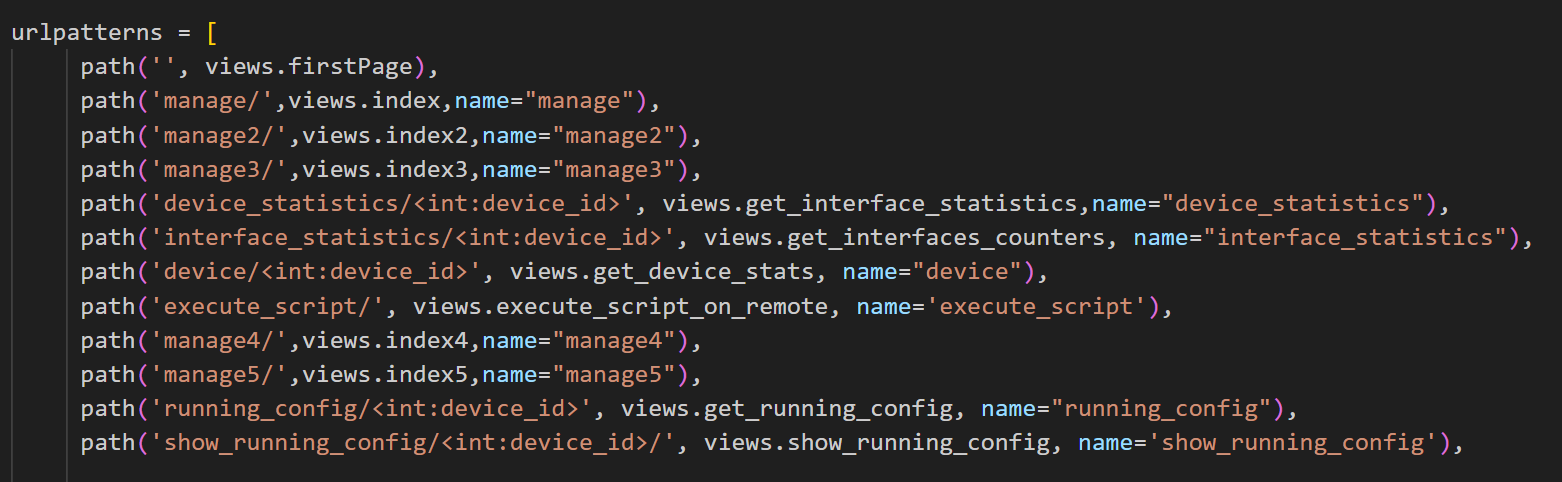
\includegraphics[width=0.9\textwidth]{graphics/urlpy.png}
	\caption{\en{url.py} }
\end{figure}

Οι συναρτήσεις σε ένα αρχείο \en{views.py} καλούνται όταν η δεδομένη διεύθυνση \en{URL} που αποστέλλεται από το
χρήστη ταιριάζει με το αντίστοιχο μοτίβο \en{URL} στο αρχείο \en{urls.py}. Παράμετροι που αποστέλλονται μέσω κλήσης
\en{HTTP} εισέρχονται στην αντίστοιχη συνάρτηση μέσω παραμέτρων ή σώματος αίτησης. Στο αρχείο \en{views.py} του \en{API}, η συνάρτηση εκτελεί το σενάριο
κώδικα με τις δεδομένες παραμέτρους εισόδου. Όταν τελειώσει η εκτέλεση του κώδικα δέσμης ενεργειών,
το αποτέλεσμα επιστρέφεται στη συνάρτηση \en{views} και μεταβιβάζεται ως πλαίσιο στο αντίστοιχο αρχείο \en{.html} για την εμφάνιση των αποτελεσμάτων στον χρήστη που εκτέλεσε το σενάριο.
Ένα παράδειγμα μιας συνάρτησης σε ένα αρχείο \en{views.py} μπορείτε να δείτε στο σχήμα παρακάτω

\begin{figure}[htb]
	\centering
	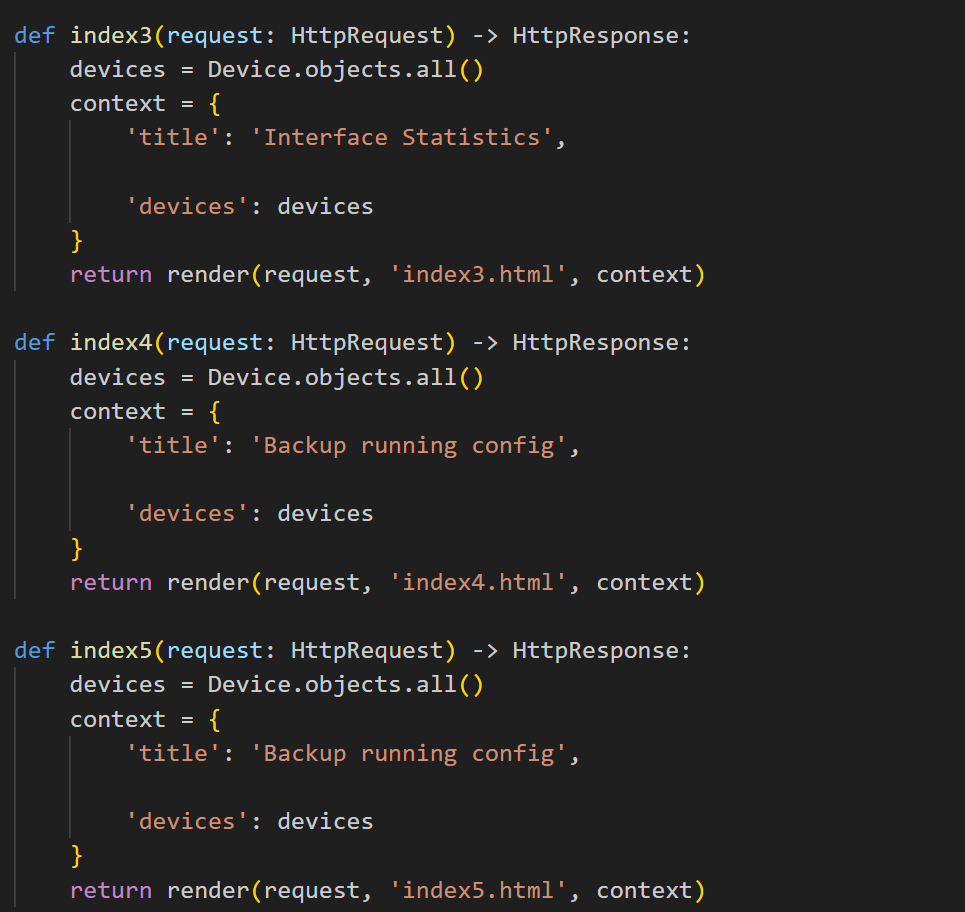
\includegraphics[width=0.9\textwidth]{graphics/viewspy.png}
	\caption{\en{views.py} }
\end{figure}

\subsection{\en{User Interface (Templates)}}
Στη συνάρτηση \en{views.py}, το \en{Django} αποδίδει το αντίστοιχο πρότυπο \en{.html}
αρχείο με ένα συγκεκριμένο πλαίσιο. Το πλαίσιο είναι σε μορφή \en{JavaScript Object Notation (JSON)} και αποστέλλεται στο αρχείο \en{.html}. Τα δεδομένα στο πλαίσιο εμφανίζονται
στο \en{.html}, εάν το \en{.html} έχει παραμετροποιηθεί κατάλληλα. Ένα παράδειγμα \en{.html} με
τον συντακτικό κώδικα για τον τρόπο πρόσβασης στα δεδομένα του πλαισίου παρουσιάζεται στην εικόνα παρακάτω



\begin{figure}[htb]
	\centering
	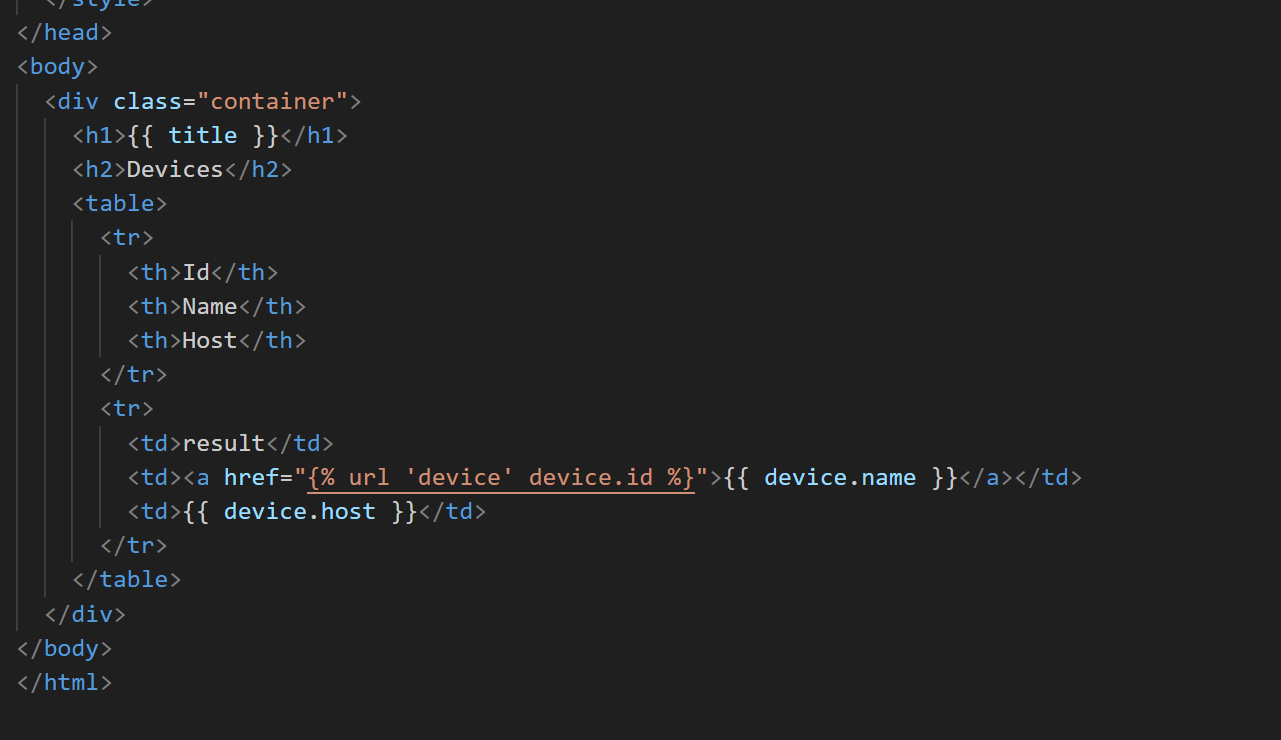
\includegraphics[width=0.9\textwidth]{graphics/html_template.png}
	\caption{Παράδειγμα \en{html} αρχείου }
\end{figure}


\section{\en{REST API Integration} και διασύνδεση με το \en{SSH protocol}}

Το \en{REST API Integration} διαδραματίζει κρίσιμο ρόλο στη 
διπλωματική εργασία, καθώς επιτρέπει την αλληλεπίδραση μεταξύ των 
διαφόρων συστημάτων και την ανταλλαγή δεδομένων μέσω του διαδικτύου. 
Το \en{REST} (\en{Representational State Transfer}) είναι μια 
αρχιτεκτονική προσέγγιση που χρησιμοποιεί τα πρωτόκολλα \en{HTTP} 
για την εκτέλεση λειτουργιών όπως η ανάκτηση, η δημιουργία, η 
ενημέρωση και η διαγραφή δεδομένων. Με την υλοποίηση \en{REST APIs}, 
καθίσταται δυνατή η διαλειτουργικότητα της εφαρμογής με άλλες 
υπηρεσίες, διευκολύνοντας τη σύνθεση πολύπλοκων λειτουργιών από 
διάφορες πηγές. Στο πλαίσιο της διπλωματικής, το \en{REST API} 
χρησιμοποιείται για την διαχείριση δικτυακών συσκευών, παρακολούθηση 
στατιστικών, εκτέλεση εντολών, διασφαλίζοντας την ασφάλεια και την 
αποδοτικότητα της επικοινωνίας μέσω διαφανών και επεκτάσιμων 
τεχνολογιών. Το \en{REST} δεν χρησιμοποιείται για την επικοινωνία της εφαρμογής
και των συσκευών αλλα εσωτερικά ως μηχανισμός δρομολόγησης προκειμένου ο χρήστης
να μπορεί να φέρει στον χρήστη το σωστό αποτέλεσμα. Η διαχείρηση των δικτυακών
συσκευών γίνεται με το πρωτόκολλο \en{SSH}.

Προσπαθώντας μέσα από το \en{wireshark} να πιάσουμε την κίνηση μεταξύ
\en{WSL} και δικτυακής συσκευής κάναμε το παρακάτω πείραμα προκειμένου να κατανοήσουμε 
πως επικοινωνεί η εφαρμογή με τις συσκευές.

Πατάμε το κουμπί \en{R1 Testing} 
και στο \en{Wireshark} κάνουμε \en{capture}
το \en{interface eth0} του \en{WSL} προκειμένου να δούμε τι γίνεται όταν εμείς πατάμε
το κουμπί για μια λειτουργία. Στο παρακάτω \en{trace} φαίνεται τι γίνεται:

\begin{figure}[htb]
	\centering
	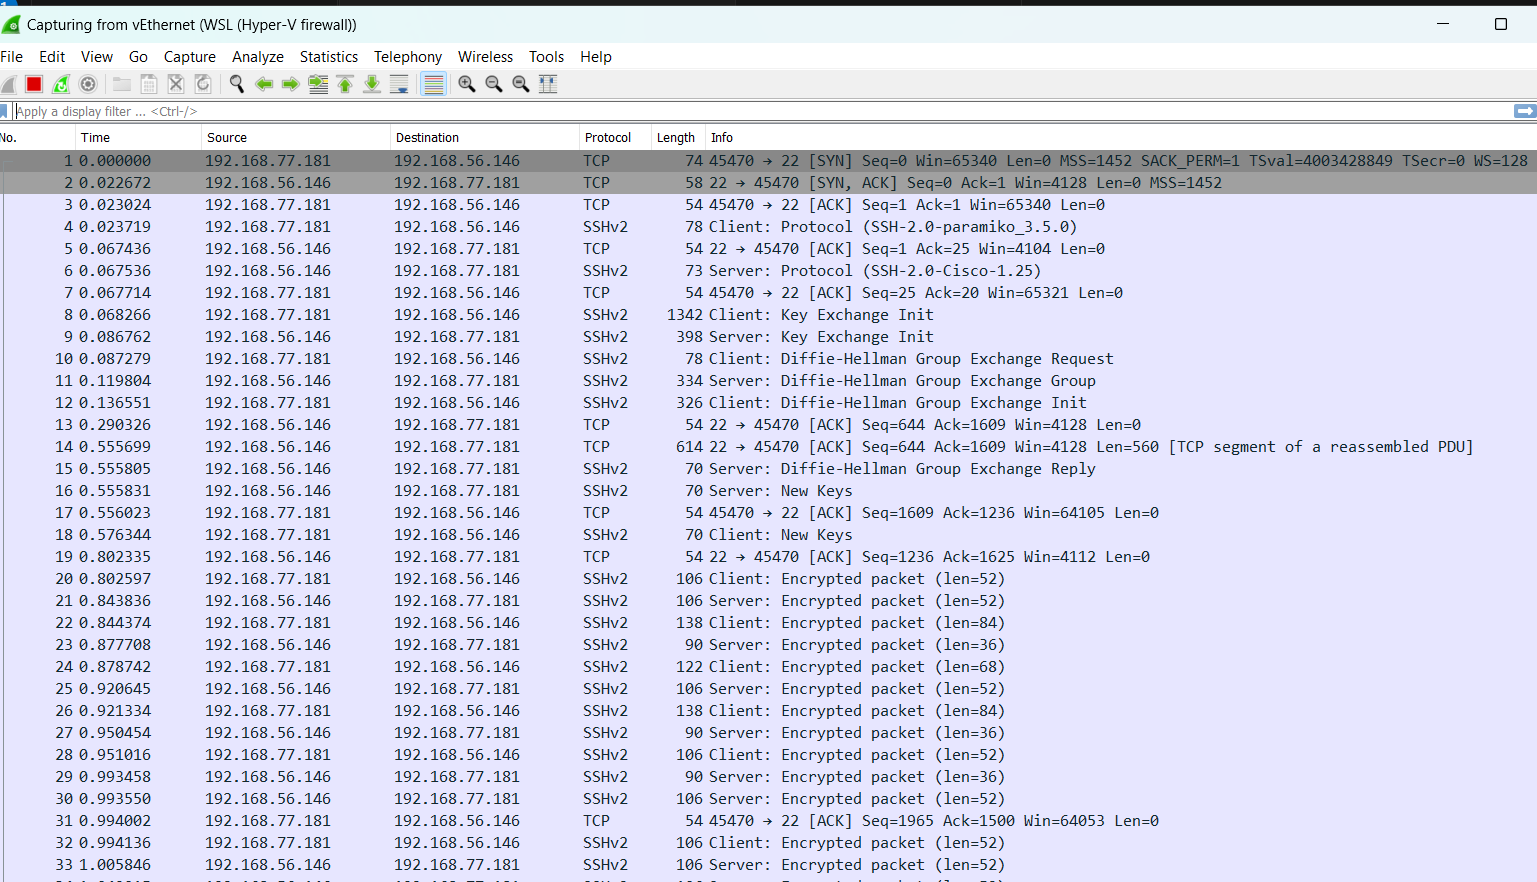
\includegraphics[width=0.9\textwidth]{graphics/wireshark.png}
	\caption{Παράδειγμα \en{wireshark} }
\end{figure}

Αυτή η αλληλουχία αντιπροσωπεύει μια τυπική ασφαλή σύνδεση \en{SSH}. Εγκαθίδρυση \en{TCP} σύνδεσης (\en{SYN,SYN/ACK,ACK}). Μετά ακολουθεί η
διαπραγμάτευση πρωτοκόλλου \en{SSH} και στο τέλος η έναρξη της κρυπτογραφημένης επικοινωνίας την οποία δε μπορούμε να δούμε. Όμως μπορούμε να δούμε τι επιστρέφεται 
απο το \en{cli} του \en{Django server} στην παρακάτω εικόνα.


\begin{figure}[htb]
	\centering
	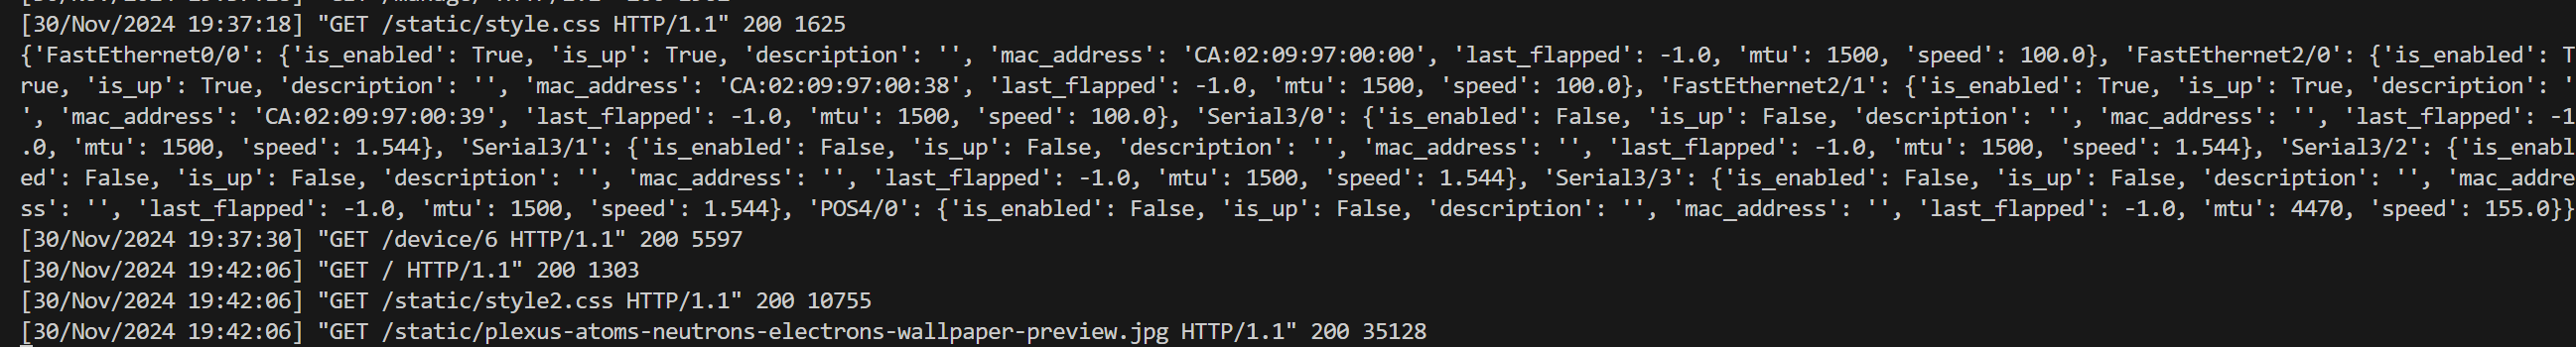
\includegraphics[width=0.9\textwidth]{graphics/rest.png}
	\caption{Απάντηση συσκευής}
\end{figure}


\section{Διασύνδεση με το \en{GNS3}}

Παρακάτω θα παρουσιαστούν τα βήματα που ακολουθήθηκαν προκειμένου να μπορέσει να μιλήσει το τοπικό δίκτυο με
το δίκτυο των εικονικών συσκευών. Προκειμένου να γίνει η σύνδεση της εφαρμογής με το \en{GNS3} γίνανε αρκετές
ρυθμίσεις.

Πρώτα σε επίπεδο συνδεσιμότητας. Σύνδεση μεταξύ \en{IOU2} και \en{Cloud}.
Το \en{IOU2} είναι ένα \en{Switch} το οποίο θα μας βοηθήσει να έχουμε επαφή με \en{L3 Devices}
αφού όλες οι συσκευές που ενώνονται μαζί του είναι στο ίδιο \en{L2 network}
Το \en{cloud} αναπαριστά το τοπικό \en{router} μας. Είναι η επαφή μας με το τοπικό δίκτυο του
\en{GNS3 server.} Λόγω αυτού θα μπορέσει ο διακομιστής που τρέχει στο \en{WSL} περιβάλλον
να επικοινωνήσει με τις συσκευές στο \en{GNS3}. Παρατίθεται το \en{cloud configuration}:

\FloatBarrier

\begin{figure}[htb]
	\centering
	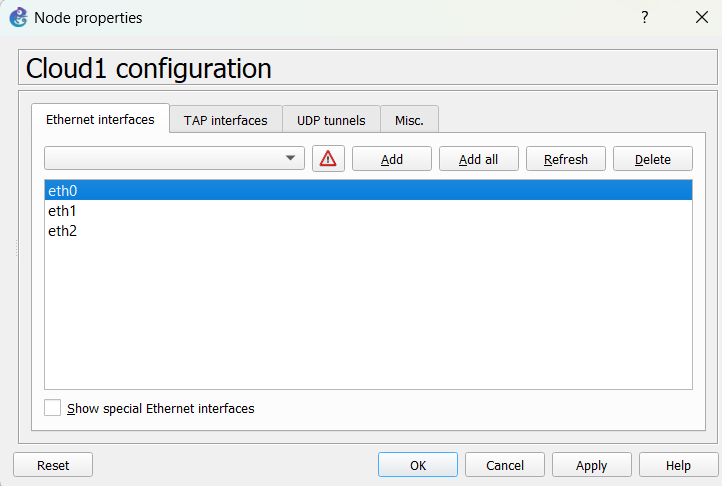
\includegraphics[width=0.9\textwidth]{graphics/cloud_configuration.png}
	\caption{Παραμετροποίηση \en{cloud}}
\end{figure}

\FloatBarrier

Δεξί κλικ και πατάμε παραμετροποίηση. Εκεί κάνουμε προσθήκη το \en{eth0} ως διεπαφή
επικοινωνίας του τοπικού δικτύου με τον διακομιστή. Το \en{eth0} είναι κρίσιμης σημασίας επιλογή
και ο λόγος που το επιλέγουμε είναι διότι στο \en{GNS3 VM} το \en{eth0} έχει την παρακάτω παραμετροποίηση.

\begin{figure}[htb]
	\centering
	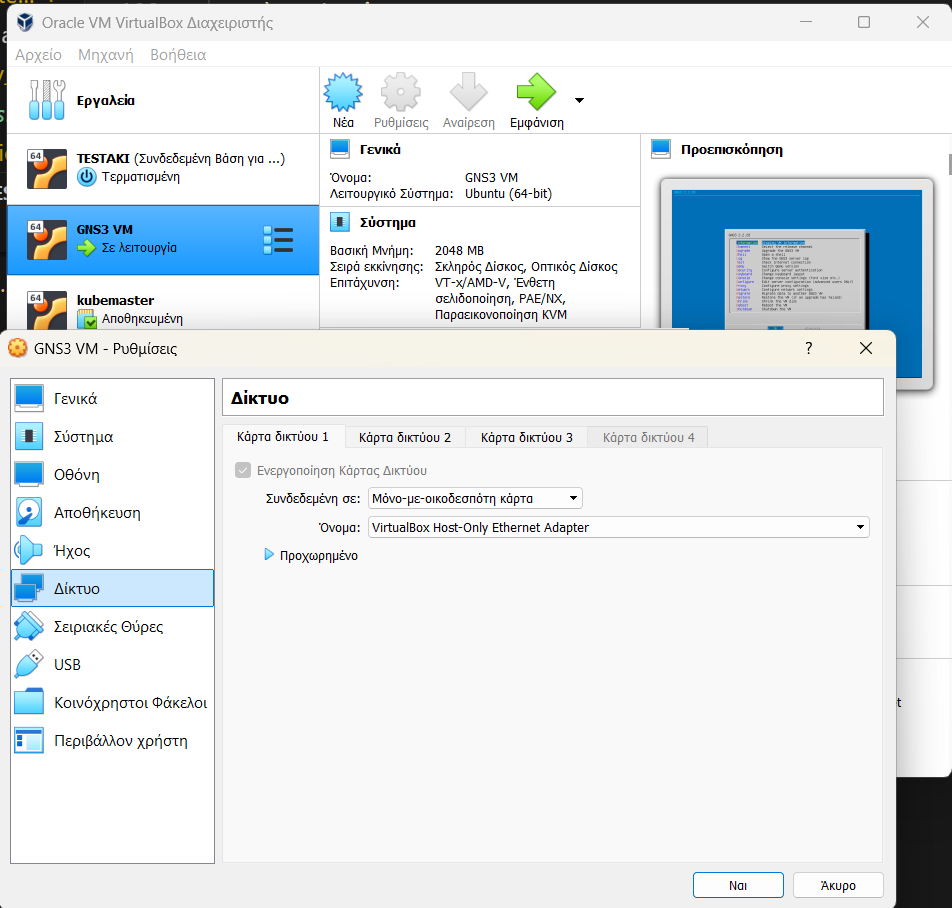
\includegraphics[width=0.9\textwidth]{graphics/eth0.png}
	\caption{Παραμετροποίηση \en{eth0}}
\end{figure}


Συνεπώς επειδή αναπαριστά μια κάρτα δικτύου η οποία συνδέει την εικονική μας μηχανή
με τον υπολογιστή στον οποίο εκτελείται αυτή. Συνεπώς οι συσκευές οι οποίες συνδέονται με το 
\en{cloud} θα έχουν απευθείας σύνδεση και με το τοπικό μας δίκτυο. 

Προκειμένου τώρα οι συσκευές αυτές να μπορέσουν να μιλήσουν με το τοπικό μας δίκτυο
θα πρέπει να τους ορίσουμε \en{IP } διευθύνσεις. Παρακάτω φαίνεται η παραμετροποίηση που έγινε 
στη συσκευή προκειμένου να πάρει \en{IP } διευθύνση από το τοπικό μας δίκτυο(192.168.56.0/24)

\FloatBarrier

\begin{figure}[htb]
	\centering
	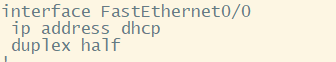
\includegraphics[width=0.9\textwidth]{graphics/dhcp_cisco_config.png}
	\caption{Παραμετροποίηση \en{DHCP}}
\end{figure}

\FloatBarrier

Έλεγχος ότι μπορούμε να επικοινωνήσουμε με τις εικονικές συσκευές της \en{Cisco}

\FloatBarrier

\begin{figure}[htb]
	\centering
	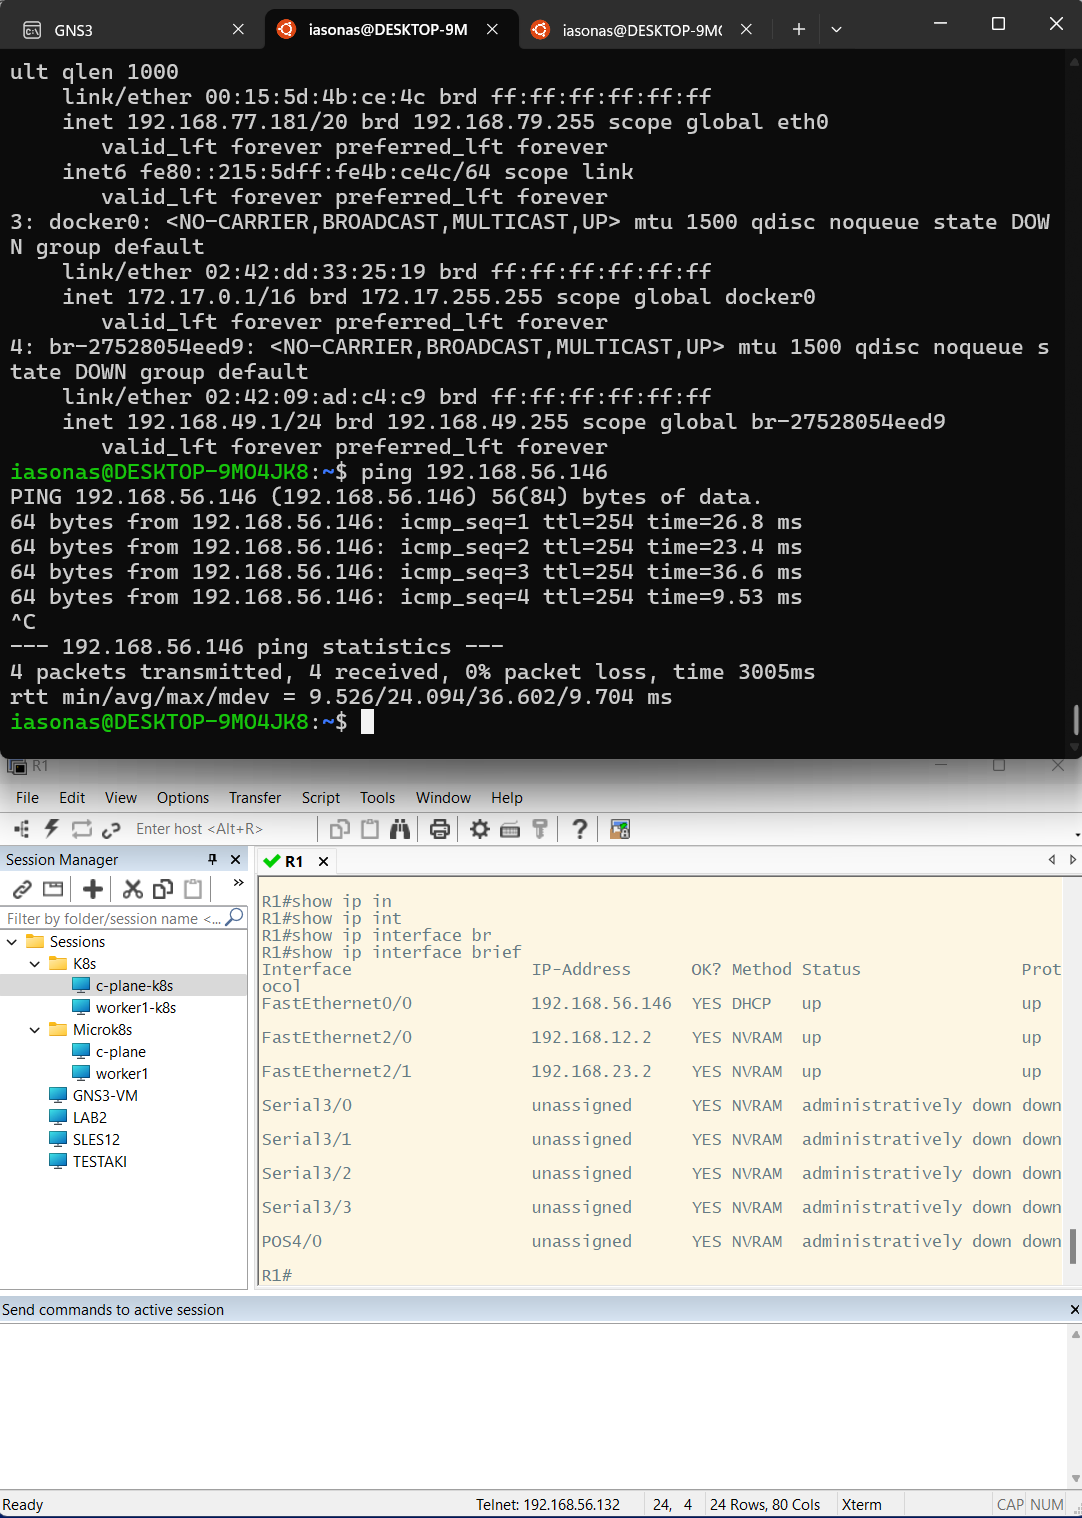
\includegraphics[width=0.9\textwidth]{graphics/test_ip_connectivity.png}
	\caption{\en{IP connectivity test}}
\end{figure}

\FloatBarrier

%\begin{equation}
%	y = \alpha x + \beta
%\end{equation}

%Αντίθετα με αυτό που θεωρεί η πλειοψηφία, το \en{Lorem Ipsum} δεν είναι απλά ένα τυχαίο κείμενο. Οι ρίζες του βρίσκονται σε ένα κείμενο Λατινικής λογοτεχνίας του 45 π.Χ., φτάνοντας την ηλικία του πάνω από 2000 έτη.


%\begin{figure}[htb]
%	\centering
%	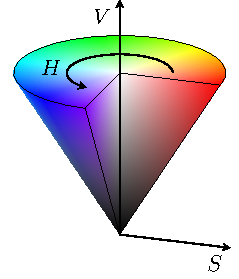
\includegraphics{tikz/hsv_cone/hsv_cone.pdf}
%	\caption{Ο χρωματικός χώρος \en{HSV}.}
%\end{figure}
